\chapter{Simultaneous Localization and Planning}\label{chap:localization-and-planning}

\todo[inline]{Rework according to results}

Typically, robot localization and motion planning are treated as mostly
independent tasks. Often, the problem provides the agent with a focused initial
belief or allows the agent to quickly reduce uncertainty by first collecting
a series of measurements that don't require elaborate motion planning. This is
particularly the case if the state space is well observed, i.e. there exists
a sensor that provides the robot with a (noisy) position reading (e.g. GPS).
For these well behaved problems, a simple yet effective approach is to first
collect sensor data while executing a default motion, i.e. rotating about the
yaw axis to collect measurements in all directions. Once state uncertainty is
reduced to a focused, unimodal belief, the problem is treated as fully observed
problem and motion planning is performed on expectation. That is, trajectories
are planned based on the assumption that the expectation of the belief, $E[b]$,
is a sufficient approximation for the true position of the robot. Furthermore,
higher statistical moments \todo{What is the right word for this?} may be used
to trigger additional information gathering. In even simpler problems, plan
execution may implicitly yield sufficient information gathering, rendering
explicit consideration of this aspect obsolete.

However, more challenging problems are obtained when information gathering
happens less naturally. In these cases, a simple approach as outlined above
may not perform well. Instead, persistently good performance requires the agent
to consider the full belief distribution as well as future observations in
order to identify informative action sequences.

\todo[inline]{Rewrite once structure (below) has converged}
An instance of such problem is studied in this chapter. We begin by stating the
problem details in \cref{sec:lp-problem-statement}.
\cref{sec:lp-pomdp-formalization} then formalizes this problem as a \ac{pomdp}.
\cref{sec:lp-solutions} presents solution strategies based on \ac{pomdp}
solvers introduced in \cref{sec:online-pomdp-solvers}, as well as two heuristic
baseline approaches. Finally, we evaluate the performance of each solver and
discuss the results in \cref{sec:lp-evaluation}.

\section{Problem Statement}\label{sec:lp-problem-statement}

In this chapter we study an instance of simultaneous localization and planning.
Consider a robot operating in a planar, previously mapped room as depicted in
\cref{fig:roomba-env}. In this figure the red marker denotes the true position
of the robot, while the blue particles represent the robot's belief of it's
current location in the room. The agent is tasked to reach the exit (green)
while avoiding falling down the stairs (red). Additionally, unnecessary
collisions are to be avoided. The scene shows the simulation in it's initial
configuration: The robot starts at a position drawn uniformly at random from
the set of all possible position-orientation tuples. This initial position is
not known by the agent, thus the particles representing the initial belief are
spread uniformly across the entire room. The robot is equipped with a single
sensor that provides information about collisions with walls of the room. The
robot's dynamics are governed by an underactuated first-order model that allows
the robot to translate forward and/or rotate about it's vertical axis. The
agent holds control authority to choose translation and rotation rates.

This problem has originally been published under the name \emph{"Escape
Roomba"} by the \emph{Stanford Intelligent Systems Laboratory} as part of the
class \emph{Decision Making under
Uncertainty}\footnote{\url{https://web.stanford.edu/class/aa228/cgi-bin/wp/}}.
The experiments presented in the following have been conducted using the
\pomdpsjl implementation of the
problem\footnote{\url{https://github.com/sisl/AA228FinalProject}}.

\begin{figure}[htpb]
  \centering
  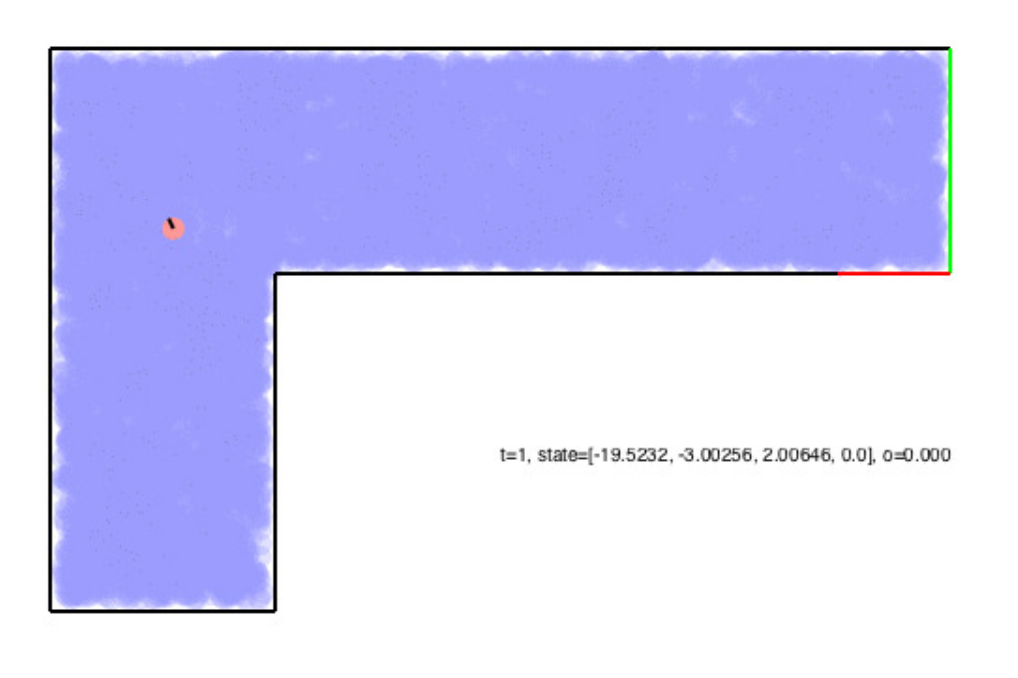
\includegraphics[width=0.7\textwidth]{roomba_demo/roomba-initial.png}
  \caption{A screen shot of the simulation environment for the \emph{"Escape
  Roomba"} problem provided by the \emph{Stanford Intelligent Systems
  Laboratory} as part of the class \emph{Decision Making under Uncertainty}.}
  \label{fig:roomba-env}
\end{figure}

\clearpage
\section{POMDP Formalization}\label{sec:lp-pomdp-formalization}

The problem is formalized as a \ac{pomdp} with the following properties introduced in \cref{sec:pomdp}:

\todo[inline]{Mention somewhere that we discretize the action space because
samples are expensive (problem setup is quite slow)}

\begin{description}
	\item[State Space $\sspace$.] The state of the robot is defined as the
	position, orientation tuple, $s=((x,y), \alpha)$. Respectively, $\sspace$ is
	the set of all positions-orientation tuples inside the room.
	\item[Action Space $\aspace$.] An action is defined as a translation-rotation
		rate tuple, $a=(v, \omega)$. $\aspace$ is the set of all these
		tuples adhering to the physical limitations of the system.
  \item[Transition Model $\tdist$.] The robot transition follows the dynamics of
    a simple differential drive model. The details of this transition are
    defined implicitly by the simulator and are treated as a generative black
    box model.
  \item[Reward Function $\reward: \sspace \times \aspace \times
    \sspace \to \reals$.] The reward model is defined as:
    \begin{equation}
      \reward(s, a, s') = r_\text{time} + \chrond_\text{collision}(s') r_\text{collision} + \chrond_\text{goal}(s') r_\text{goal} + \chrond_\text{stairs}(s') r_\text{stairs}.
    \end{equation}
    Here, $\chrond_\text{c}(s)$ denotes the \vname{Kronecke delta} function under the condition, \vname{c}, such that
    \begin{equation}
      \chrond_\text{c}(s) = \begin{cases}
        1, & \text{if condition $c$ holds for $s$}\\
        0, & \text{otherwise.}
      \end{cases}
    \end{equation}
    The reward model is parametrized by the following
    quantities: $r_\text{time}$ is a living penalty encouraging the robot to
    minimize the time until the goal is reached; $r_\text{collision}$ is
    a penalty for collision with walls; $r_\text{goal}$ is the reward obtained
    when reaching the goal, and $r_\text{stairs}$ the penalty for falling down
    the stairs.\\
  \item[Discount Factor $\gamma$.] Rewards are discounted with $\gamma = 0.99$.
  \item[Observation Space $\ospace$.] The sensor provides a binary output,
    stating whether the robot is currently in contact with the wall or not. That
    is, there are only two observations: $o^0$  and $o^1$.
  \item[Observation Model $\odist$.] The collision sensor is deterministic.
    That is, the observation model is a Dirac delta function, evaluating
    non-zero for a state, $s$, if and only if the collision feature evaluated
    on $s$ matches the observation, $o$.
\end{description}

Summarizing, the problem is a \ac{pomdp} with continuous state and action space
and a discrete observation space. The reward model chosen for this problem is
sparse. That is, it only encodes high level preferences but avoids biasing the
solution through additional transition dependent rewards (e.g. rewards for
reducing the distance to the goal).

\section{Solution Strategies}\label{sec:lp-solutions}

We solve the \ac{pomdp} described in \cref{sec:lp-pomdp-formalization} using
\ac{despot} and \ac{pomcpow}, respectively. For each of these solvers we
propose two domain specific adaptations to guide the policy search. In addition
to that, we present two baseline policies that use a heuristic policy to
control the agent. In order to consider efficiency of each algorithm we limit
the computation time per planning step to $T_\text{max} = \SI{1}{s}$. Each
policy uses the same particle filter to estimate the root belief.
\todo[inline]{Maybe point to code attached or to repo.}

\subsection{Baseline Policies}\label{sec:lp-baseline}

In order to obtain a baseline we make a common simplifying assumption: Instead
of planning with the full root belief, $b$, the policy uses only the \emph{most
likely state}, $\sml = \mode(b)$. Using this approximation, the problem is then
treated as fully observable. That is, at every time step the control action is
selected based on the assumption that the true position of the robot matches
the most likely state. The loop is closed by applying only the first action of
the policy at each time step to then update the belief and re-plan from the
next most likely state, $\sml' = \mode(b')$. Based on this assumption we
propose two heuristic policies:

\begin{description}
  \item[\ac{mlra}] For this baseline, the agent uses a simple, handcrafted
  feedback policy that does not involve any active reasoning about future
  states. Instead, it uses a proportional controller to track the center line
  of the room to reach exit. As a result, evaluating \ac{mlra} is
  computationally inexpensive. \ac{mlra} is not an optimal policy for the fully
  observable problem.
  \item[\ac{mlmpc}] This planning agent computes the optimal state trajectory
  for the fully observable problem starting from $\sml$ using \ac{mpc}. That
  is, it uses the negative reward model as a cost function to obtain the
  objective for the \ac{mpc}.
\end{description}

Unlike \ac{mlra}, \ac{mlmpc} is an optimal policy for the fully observed
problem. However, it should be noted that this result does not necessarily
translate to the partially observed domain. Appendix TODO\todo{cref to
appendix} compares the performance of both baseline policies for the fully
observable case.

\subsection{POMDP Solvers}\label{sec:lp-planners}

We use \ac{despot} and \ac{pomcpow} to solve the \ac{pomdp}. For each solver we
propose two strategies in which domain knowledge can be utilized to guide the
policy search for the localization and planning problem.

\subsubsection{DESPOT}\label{sec:lp-planners-despot}

As presented in \cref{sec:theory-despot}, \ac{despot} uses upper and lower
bounds, $U_0$ and $L_0$, on the value function to guide the policy search and
prune the determinized policy tree. In theory, the tighter these bounds are on
the true value function, the more efficiently the algorithm will focus on
exploring the relevant trajectories. On the other hand, if these estimates
violate the true bounds on the optimal cost to go, \ac{despot} with perform
sub-optimally. However, as proven in \cite{somani2013despot}, the algorithm is
robust against approximation errors. That is, similar to informed graph search
algorithms like \emph{A*}, the performance of the algorithm will degrade
gracefully with violations of $U_0$. In fact, similar to bounded relaxations of
\emph{A*}, non-admissible heuristics may help to find good solutions earlier.
Therefore, even if $U_0$ is not a true upper bound on the optimal value, it may
help to improve performance when limited planning time does not allow to
thoroughly explore the search space. Furthermore, it should be noted that
finding tight bounds at the expense of high compute also defeats the purpose.
In the limit, finding the tightest upper and lower bound on the optimal value
requires solving the entire \ac{pomdp}. Therefore, choosing suitable upper and
lower bounds is an important design choice when adapting \ac{despot} for
a specific problem.

There exist a variety of strategies to compute these upper and lower bounds.
\todo{maybe list some common ones}
In the following we present two of the strategies we found most effective for
the problem studied here.
\todo[inline]{point to the code on the cd (or appendix)}

\begin{description}
  \item[Analytic Bounds] In this strategy we compute the bounds using an
    analytic, closed form\todo{what is a better phrasing for this?}
    approximation for $U_0$ and $L_0$. Due to the structure of the reward
    model, we can directly compute the cumulative reward for an arbitrary
    $n$-step, collision-free trajectory. Let $\hat{\Sigma}: \naturals \to
    \reals$ be this mapping. We compute the upper bound, $U_0$, on the optimal
    value by considering a strict relaxation of the problem: First, we assume
    that the robot is located at the closest position to the goal out of all
    particles in the current belief; Second, we assume that the robot can
    immediately move on a straight line to the target. With this relaxation we
    compute the minimum remaining number of steps, $n_{\text{min}}$, from the
    minimum Euclidean distance over all particles to the goal and the maximum
    translational speed. For the lower bound, $L_0$, we proceed in
    a similar fashion. In this case, however, we consider the worst case
    particle by using the $\ell_1$ norm as a distance metric combined with an
    under-approximation on the velocity to obtain $n_{\text{max}}$. In either
    case, we use $\hat{\Sigma}$ to map the step estimate to a corresponding
    return. Using these approximations, $U_0$ is a true upper bound on the
    optimal value. While for $L_0$ there is no strict guarantee to be a true
    lower bound, we found that most cases it is well behaved.
  \item[Rollout Lower Bound] This strategy uses the same upper bound as the
    first approach. However, for $L_0$ we use a default policy rollout to
    obtain a true lower bound. In order to generate a structured motion, we use
    a \emph{fixed-action} policy that always selects the forward action,
    instead of the common random policy rollout. By this means, the rollout
    policy provides a tight lower bound once evaluated from a state that
    already faces the exit of the room.
\end{description}

\subsubsection{POMCPOW}\label{sec:lp-planners-pomcpow}

\ac{pomcpow} uses a value estimate to approximate the remaining reward to be
collected from a leave node of the policy tree. Due to the design of the
algorithm, this value estimate is only ever invoked on observation nodes when
visited for the first time (cf. \cref{alg:pomcpow}). As a result, the
corresponding belief consists of only a single state and the problem is de
facto fully observable. Hence, in order to adapt this algorithm for a specific
problem one can design the value estimate based on the corresponding \ac{mdp}.
Hereafter, we present two strategies strategies to compute this value estimate
for the localization and planning problem.

\begin{description}
  \item[Analytic Value Estimate] We compute an analytic value estimate for
    state, $s$, with a strategy similar to the one used to obtain analytic
    bounds for \ac{despot}. We relax the planning problem by assuming that the
    robot can move immediately from $s$ to the goal on a rectilinear
    trajectory. Using this relaxation we can compute the estimate on the
    remaining number of steps to the goal, $\hat{n}$. We then obtain the value
    estimate for an $\hat{n}$-step, collision-free trajectory by propagating
    $\hat{n}$ through $\hat{\Sigma}$, introduced above.
  \item[Rollout Estimate] A commonly used strategy in \ac{mcts} is a random
    policy rollout \cite{browne2012survey}. For this problem, however, random
    play-outs do not provide a good value estimate since random trajectories
    will often fail to reach a terminal state within reasonable time. Instead,
    we use the \emph{fixed-action} policy proposed for the \ac{despot} lower
    bound approximation in the preceding paragraph.
\end{description}

\section{Evaluation}\label{sec:lp-evaluation}

We evaluate the performance of each strategy by running $N_\text{sim} = 1000$
simulations for every setup. In an effort to reduce sampling variance, we
initially fix $N_\text{sim}$ random seeds. These seeds are shared across the
different setups for a fixed run. By this means, the $i$th run of each setup
will see the same random outcome (i.e. same initial conditions and noise
trajectories, etc.). In order to handle cases in which the agents fails to
reach a terminal state in a reasonable amount of time, each simulation is run
for a maximum of number of time steps, $T_\text{max,sim} = 300$. The choice of
this upper bound on simulation time is justified by evaluation of the optimal
policy for the fully observable problem. In the corresponding \ac{mdp} with the
same set of initial conditions, \ac{mlmpc} reached the goal within a maximum
number of $56$ over all scenarios. Therefore, it is reasonable to assume that
a well behaved policy for this \ac{pomdp} should be able to reach a succeeding
terminal state within a time horizon more than five times longer than the worst
case fully observable run.

We begin by comparing the performance of each strategy by examining the
cumulative discounted reward. Since maximizing the sum of discounted rewards is
the objective function for this optimization function, this is the most natural
benchmark. In order to account for the reward discarded in cases where
$T_\text{max, sim}$ is exceeded, we penalize the value of these runs by
extrapolating the living penalty over infinite horizon. Since the sum over the
infinite sequence of discounted rewards is geometric series, we obtain the
closed form solution,
\begin{equation}
  r_{T_\text{sim,max}} = \sum_{t=1}^\infty r_\text{time} \gamma^{t-1} =  r_\text{time} \frac{\gamma}{1-\gamma}.
\end{equation}
Since this reward is collected at the end of the simulation horizon it must
discounted accordingly, entering the objective function as
\begin{equation}
  \Delta V_{T_\text{max,sim}} = r_{T_\text{sim,max}} \gamma^{(T_\text{max,sim} - 1)}
\end{equation}
Following this argument, with the parameters chosen for this problem an agent
that does not reach a terminal state within the simulation horizon is penalized
with $\Delta V_{T_\text{max,sim}} = -0.49$.

\Cref{fig:lp-value-sem-inf-discounted} shows the mean and \ac{sem} of the cumulative
discounted reward for $1000$ experiments over each policy. The \ac{sem}
approximates the standard error between the empirical mean obtained from the
sampled experiments and the true mean of the distribution, obtained
hypothetically for $N_\text{sim} \to \infty$. The results shows that under this
metric all \ac{pomdp} planners perform significantly better than the baseline
policies. Within the baselines the planning agent (\ac{mlmpc}) performs better
than the proposed reflex agent (\ac{mlra}). Out of all \ac{pomdp} planners
\ac{pomcpow} with analytic value estimate achieves the best results. Furthermore,
notice that \ac{despot} shows approximately the same performance for both bound
approximations while for \ac{pomcpow} the analytic value estimate shows a yields
improvement.

\begin{figure}[H]
  \centering
  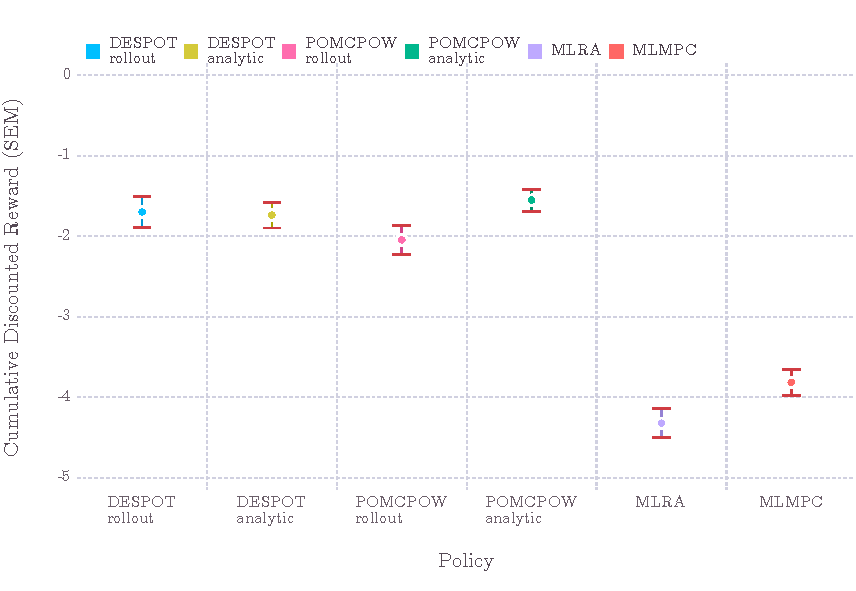
\includegraphics[scale=1.0]{roomba_plots/lp_value_sem_eval_plot-inf_discounted_reward.pdf}
  \caption{Mean and \acf{sem} for each policy introduced in \cref{sec:lp-solutions}.}
  \label{fig:lp-value-sem-inf-discounted}
\end{figure}

Further insight is gained by looking at the distribution of returns for each
policy. \Cref{fig:lp-value-violin-inf-discounted} shows an approximation of the
probability density function for the value distribution based on the $1000$
samples for each policy. From this visualization another important difference
becomes apparent. While the mean performance of all \ac{pomdp} planners is
approximately the same, those versions of \ac{despot} and \ac{pomcpow} using an
analytic strategy for bound and value approximation manage to reduce the lower
tail end of the distribution. As a result, these planners show less variance in
performance than solvers using the corresponding rollout estimates.

\begin{figure}[H]
  \centering
  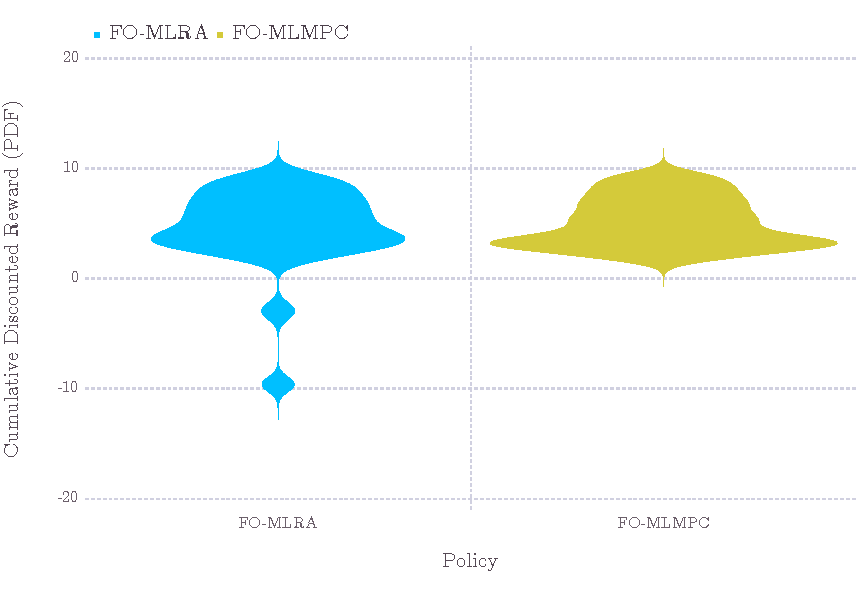
\includegraphics[scale=1]{roomba_plots/lp_value_violin_eval_plot-inf_discounted_reward.pdf}
  \caption{Approximation of the \acf{pdf} for the discounted cumulative reward
  for each policy.}
  \label{fig:lp-value-violin-inf-discounted}
\end{figure}

These quantitative results also manifest in the qualitative performance of each
policy. When looking at trajectories generated by each solver, we notice that
the \ac{pomdp} planners typically generate trajectories that efficiently
eliminate a lot of uncertainty. The baseline strategies on the other hand only
passively reduce uncertainty by colliding with wall if the mode of the belief
is located in cluster far away from the true position of the robot. For many
cases this kind of passive information gathering is strong enough to help the
robot eventually reach it's goal. However, we notice that for certain
typologies of the belief the baseline policies fail to reduce uncertainty, e.g.
if the belief is highly symmetric. In these cases, often slight modifications
of the trajectory would have been sufficient to break symmetry and completely
eliminate a cluster. While \ac{despot} and \ac{pomcpow} are able to actively
identify information gathering strategies for these cases, the baseline
policies often oscillate until repeated re-sampling in the particle filter
breaks the symmetry to an extent that allows to stabilize decisions.

Furthermore, one can observe that all \ac{pomdp} planners are significantly
better at avoiding failures (falling down the stairs). If the planner is
presented with a belief that features a cluster near the stairs, the agent
typically chooses a sequence of actions that is safe for this hypothesis and
reduces uncertainty in this regime to avoid entering the failing terminal
state. Since the baselines consider only the most likely state, these policies
fail when the topology of the reward is such that this state is facing
the goal while the true position -- guided by particles with a smaller
likelihood weight -- is facing the stairs.

Finally, we observe that the \ac{pomdp} planners using a rollout strategy to
guide the search behave more myopic. While shortsighted planning still allows
the agent to be robust against falling down the stairs, these policies tend to
get stuck when a long sequence of actions is required to eliminate uncertainty.
A possible reason for this is the fact that rollouts are more computationally
expensive than analytic bound and value estimates. Additionally, in these
regimes the fixed-action rollout typically does not provide a tight lower bound
or accurate value estimate for \ac{despot} and \ac{pomcpow}, respectively. In
the case of \ac{despot}, even though the sparse approach most likely allows
some branches of the tree to be constructed to full depth, the loose lower
bound causes policy search to be poorly guided while the limit planning time
does prevents sufficient exploration of more promising branches. In the case of
\ac{pomcpow} the computationally expensive rollout performed for every iteration
of the algorithms hinders the policy tree to reach sufficient depth within
the computation budget. Since rewards are sparse, on a short horizon all
futures appear to provide similar reward. Hence, \ac{despot} and \ac{pomcpow}
fail to identify a promising strategy within their mostly shallow policies trees.

\todo[inline]{Maybe have some figures with sequences of frames and beliefs to show
what the agent does.}

Summarizing the results of this qualitative analysis,
\emph{\ac{despot}-analytic} and \emph{\ac{pomcpow}-analytic} generate highly
efficient and robust behaviors. All other policies show weaker with different
kinds of failure modes: The rollout versions of the \ac{pomdp} planners more
often fail to reach the exit due to myopia but still show good performance when
it comes to avoiding failure states; \ac{mlmpc} rarely fails to reach the goal
state but often takes very long or becomes unlucky when greedily tyring to
reach the exit; \ac{mlra} shows an overall worse performance than all other
policies.

These results are additionally confirmed when evaluating metrics other than the
objective of the optimization problem. \Cref{fig:lp_outcome} shows a histogram
of the outcome statistics for each policy. We distinguish between three classes
of outcomes: \emph{success (+)}, the robot reached the exit; \emph{failed to
exit (0)}, the agent did not make it to the exit within the simulation horizon;
and \emph{failure (-)}, the robot fell down the stairs. Notice that
\emph{\ac{pomcpow}-analytic} succeeds in than $96.9\%$ of all runs. Given the
fact that about $3\%$ of the perimeter is covered by stairs and initially the
robot has to take a random guess to receive information, this policy can be
considered near optimal with respect to safety.

\begin{figure}[htpb]
  \centering
  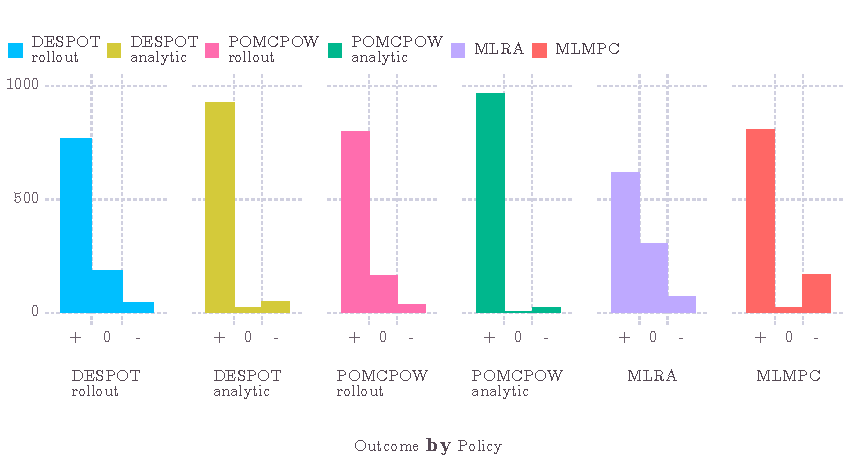
\includegraphics[scale=1.0]{roomba_plots/lp_outcome_eval_plot.pdf}
	\caption{Histogram of the outcome frequencies grouped by policy. Outcome
			     classes: \emph{success (+)}, the robot reached the exit; \emph{failed to
				   exit (0)}, the agent did not make it to the exit within the simulation horizon;
		 	 	   and \emph{failure (-)}, the robot fell down the stairs.}
	\label{fig:lp_outcome}
\end{figure}

Additional evidence for the findings discussed above is provided by the
statistics of the cumulative \emph{undiscoutned} reward. While this metric does
not match the objective for the infinite horizon formulation, it may alighn more closely with the
perceived \emph{qualitative performance} since one can only observe the agent
for a finite time horizon. \Cref{fig:lp_eval_undiscounted} depcits the \ac{sem}
and \ac{pdf} approximation for the undiscoutned reward sequence. Using this
metric, it becomes clear that the analytic versions of the \ac{pomdp} planners
outperform all other strategies. Here, we can additionally identify a subtle
performance gap between \emph{\ac{despot}-analytic} and
\emph{\ac{pomcpow}-analytic}. The \ac{pdf} approximation of the
cumulative undiscoutned reward show that \emph{\ac{pomcpow}-analytic} manages
to eliminate large parts of the low value tail.

In summary we can state that for this problem we were able to generate robust
and efficient behaviors through \ac{pomdp} planning. We show that by carefully
integrating domain knowledge in a computationally efficient manner, we obtain
policies significantly safer and more efficient than the common baseline
approaches.

\begin{figure}[htpb]
  \centering
  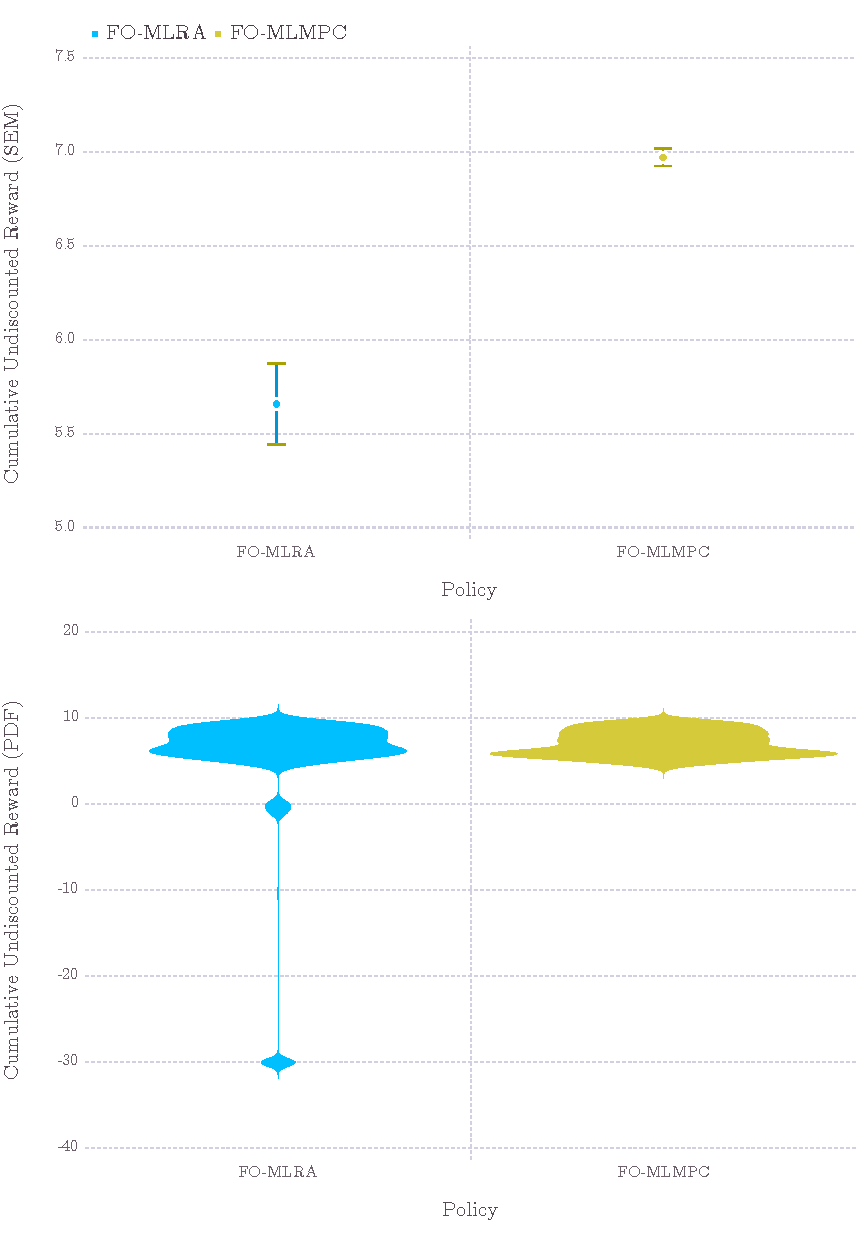
\includegraphics[scale=1]{roomba_plots/lp_value_eval_plot-undiscounted_reward.pdf}
  \caption{Statistics of the cumulative \emph{undiscounted} reward for each
  policy. Top: Mean and \acf{sem}. Bottom: Approximation of the \acf{pdf}.}
  \label{fig:lp_eval_undiscounted}
\end{figure}

%  \begin{figure}[H]
%    \centering
%    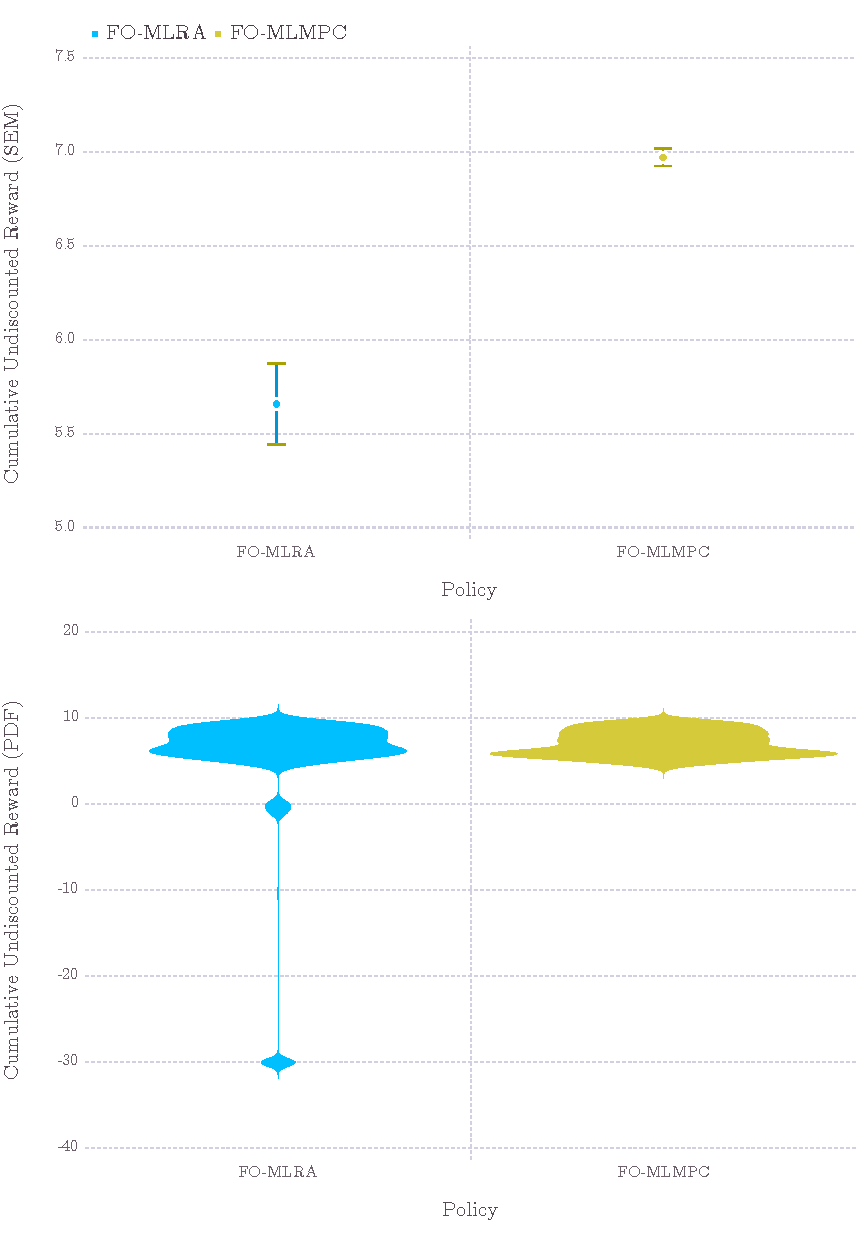
\includegraphics[scale=1]{roomba_plots/lp_value_eval_plot-undiscounted_reward.pdf}
%    \caption{Name}
%    \label{fig:name}
%  \end{figure}
